\documentclass{beamer}

\usepackage[utf8]{inputenc}
\usepackage[T1]{fontenc}
\usepackage[french]{babel}
\usepackage{amssymb}
\usepackage{amsmath}
\usepackage{mathrsfs}
\usepackage{graphicx}
\usepackage{verbatim}
\usepackage{multimedia}

\title[Projet Robotique Autonome]{Optimisation de la marche de Sigmaban}
\author{Maxime Carrere, Quentin Maouhoub, Quentin Rouxel}
\institute{}
\date{31/01/2013}

\usetheme{Madrid}
\usecolortheme{beaver}
\useinnertheme{circles}
\setbeamertemplate{blocks}[rounded][shadow=false]
\setbeamertemplate{caption}[numbered]
%\setbeameroption{show notes}
%\setbeamercovered{transparent}

\begin{document}

\begin{frame}
    \titlepage
\end{frame}

\begin{frame}{Sigmaban}
    \begin{itemize}
        \item 20 servos moteurs
        \item 2 accéléromètres, 2 gyroscopes
        \item 4 capteurs de pressions par pieds
        \item Rhoban Serveur sur le mini pc embarqué
    \end{itemize}
\end{frame}

\begin{frame}{Création des mouvements}
    \begin{itemize}
        \item Utilise l'interface graphique de Rhoban
        \item Stabilisation (boucle de contrôle proportionnel et proportionnel intégrale)
        \item Primitives motrices sinusoïdales. Paramètres : fréquence, gain et phase des signaux
    \end{itemize}
\end{frame}

\begin{frame}{Test de la marche sur Sigmaban}
    \movie[scale=0.3,showcontrols,poster]{video sigmaban}{sigmaban.avi}
\end{frame}

\begin{frame}{Capteurs}
    \begin{figure}[h]
        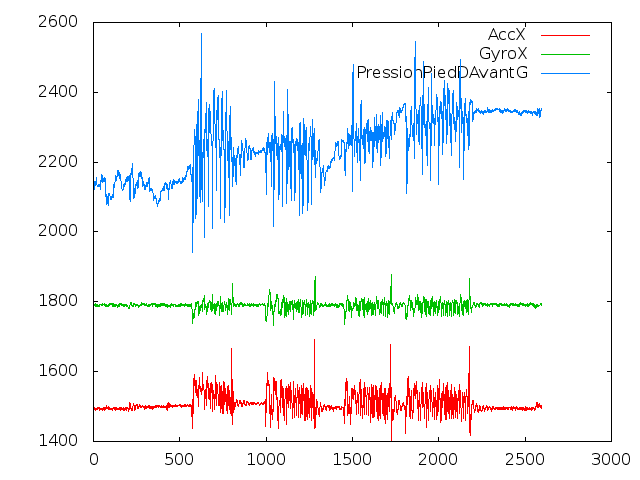
\includegraphics[scale=0.4]{../report/sensors.png}
        \caption{Valeur brute de trois capteurs au cours de l'enregistrement}
    \end{figure}
\end{frame}

\begin{frame}{Détection des temps de marche}
    \begin{figure}[h]
        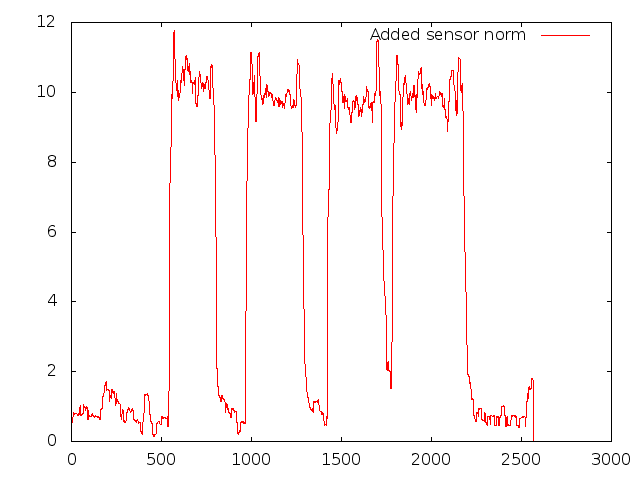
\includegraphics[scale=0.4]{../report/walks.png}
        \caption{Norme (max amplitude) de tous les capteurs sommés. Détection des phases de marche}
    \end{figure}
\end{frame}

\begin{frame}{Analyse par FFT d'un capteur}
    \begin{figure}[h]
        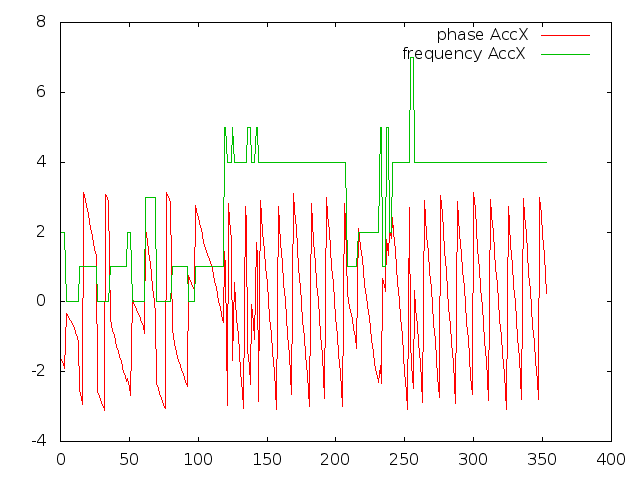
\includegraphics[scale=0.4]{../report/phase_freq.png}
        \caption{Phase et fréquence (fondamentale) d'un capteur au cours d'une des marches}
    \end{figure}
\end{frame}

\begin{frame}{Résultats de la fonction Fitness}
    \begin{figure}[h]
        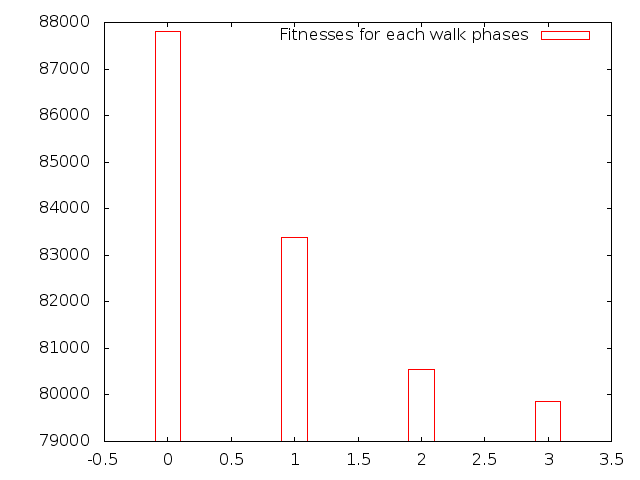
\includegraphics[scale=0.4]{../report/fitnesses.png}
        \caption{Valeur de la fonction de récompense pour les quatres marches}
    \end{figure}
\end{frame}

\begin{frame}{Apprentissage}
    \begin{block}{Algorithme \text{particulaire}}
        \begin{itemize}
            \item Entrée : un ensemble de n listes de p paramètre chacune
                    leurs fitness respectives
            \item Sortie : un ensemble de n listes générées à partir des mieux notées.   
        \end{itemize}
    \end{block}
\end{frame}

\begin{frame}{Conclusion}
    \begin{itemize}
        \item Les tests restent à faire
        \item Tester si la fonction fitness discrimine deux jeux de paramètres
        \item Paramètres à tester dans le calcul de la fonction Fitness (FFT)
        \item Normalisation des valeurs des capteurs dans Rhoban Server
        \item Prise en compte des autres harmoniques du spectre et de l'amplitude
            des capteurs
    \end{itemize}
\end{frame}

\begin{frame}{Annexe 1}
    \begin{figure}[h]
        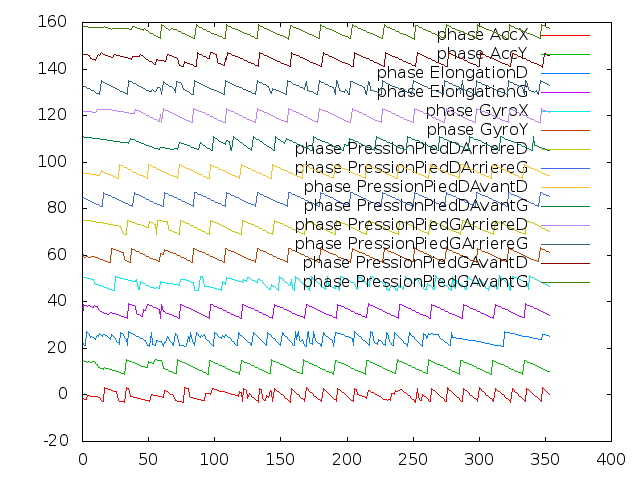
\includegraphics[scale=0.4]{../report/all_sensor_phases.png}
        \caption{La phase de tous les capteurs au cours d'une des marches}
    \end{figure}
\end{frame}

\begin{frame}{Annexe 2}
    \begin{figure}[h]
        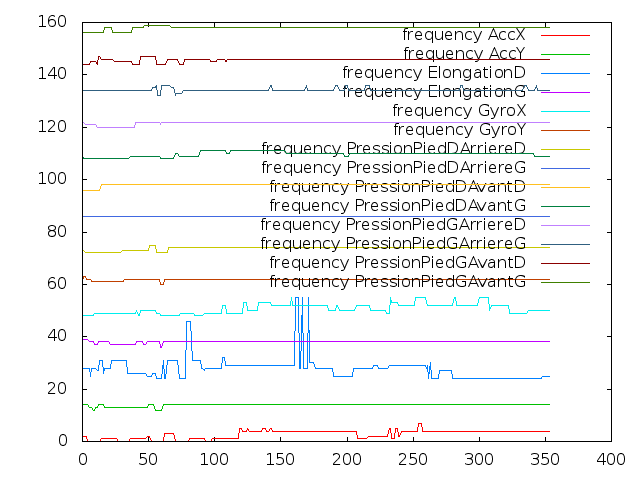
\includegraphics[scale=0.4]{../report/all_sensor_freq.png}
        \caption{La fréquence de tous les capteurs au cours d'une des marches}
    \end{figure}
\end{frame}

\end{document}

